%! Licence = CC BY-NC-SA 4.0

%! Author = gianfluetsch
%! Date = 22. Jan 2022
%! Project = icth_summary

\section{Signal-to-Noise Ration und Pegelplan}

\subsubsection{Prüfung HS2018}
Ein drahtgebundenes Übertragungssystem hat eine Systembandbreite B = 2 GHz.\\

\textbf{Wie gross ist die thermische Rauschleistung [in dBm] in dieser Systembandbreite? Bitte Herleitung angeben, nicht nur numerisches Endresultat.}\\
$N=-174dBm+10logB=-174dBm+10log(2*10^9)$\\
$N=-174dBm + 3 dB + 90 dB = -81dBm$\\

Der Empfänger in diesem Übertragungssystem besteht aus einem Bandpassfilter mit 2 GHz Bandbreite und 2 dB Einfügungsdämpfung und einem nachgeschalteten Mischer
mit 8 dB Einfügungsdämpfung. Es sollen folgende Randbedingungen gelten:\\
\begin{itemize}
    \item Der Signal-zu-Rauschabstand (SNR) an jeder Stelle des Pegelplans soll mindestens +20 dB betragen, damit eine geringe Bitfehlerrate garantiert ist.
    \item Der maximale Signalpegel am Eingang des Mischers darf maximal +5 dBm betragen, damit nicht zu viele ungewollte Mischprodukte entstehen.\\
\end{itemize}

Tragen Sie diese beiden Randbedingungen in den untenstehenden Pegelplan ein und bestimmen Sie anschliessend grafisch im Pegelplan den Verlauf für den minimalen und
maximalen Pegel:
\begin{center}
    \vspace{-8pt}
    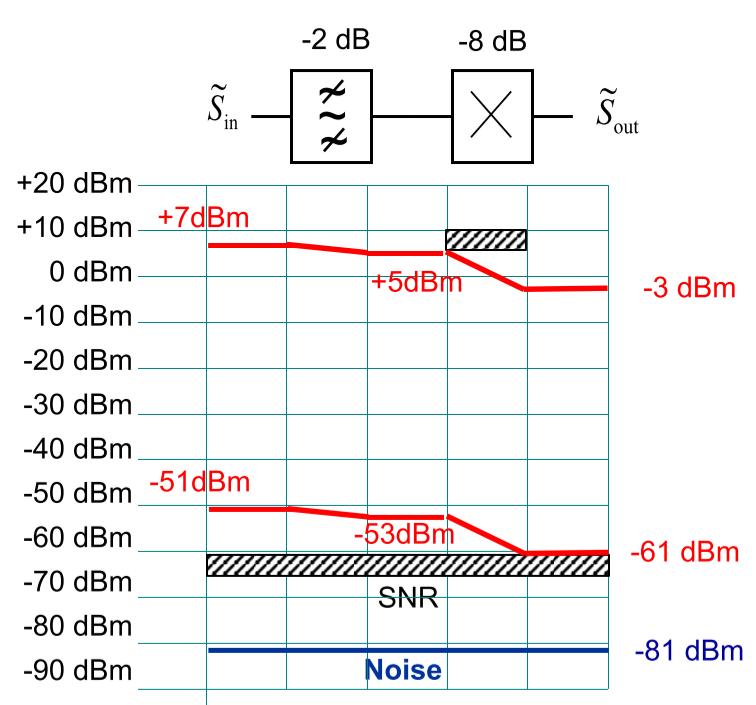
\includegraphics[width=.6\linewidth]{./11-pegelplan/hs2018}
    \vspace{-8pt}
\end{center}

\textbf{Wie gross werden gemäss des obenstehenden Pegelplans der maximale und minimale Pegel [in dBm] am Eingang des Empfängers und welche Signaldynamik [in dB] resultiert?}\\
$S_{max}=+7dBm$\\
$S_{min}=-51dBm$\\

$Signaldynamik = S_{max}-S_{min}=+7dBm+51dBm=58dB$

\columnbreak

\subsubsection{Prüfung HS2017}
Ein drahtloses Übertragungssystem hat eine Systembandbreite B = 80 MHz.\\

\textbf{Wie gross ist die thermische Rauschleistung [in dBm] in dieser Systembandbreite? Bitte Herleitung angeben, nicht nur numerisches Endresultat.}\\
$N=-174dBm+10logB=-174dBm+10log(2*2*2*10^7)$\\
$N=-174dBm + 3 dB + 3 dB + 3 dB + 70 dB = -95dBm$\\

Der Empfänger in diesem drahtlosen Übertragungssystem besteht aus einem Bandpassfilter mit 80 MHz Bandbreite und 3 dB Einfügungsdämpfung und einem nachgeschalteten
Verstärker mit 30 dB Verstärkung. Es sollen folgende Randbedingungen gelten:\\
\begin{itemize}
    \item Der Signal-zu-Rauschabstand (SNR) an jeder Stelle des Pegelplans soll mindestens +15 dB betragen, damit eine geringe Bitfehlerrate garantiert ist.
    \item Der maximale Signalpegel am Ausgang des Verstärkers soll maximal +10 dBm betragen, damit keine Signalverzerrungen auftreten\\
\end{itemize}

Tragen Sie diese beiden Randbedingungen in den untenstehenden Pegelplan ein und bestimmen Sie anschliessend grafisch im Pegelplan den Verlauf für den minimalen und
maximalen Pegel:
\begin{center}
    \vspace{-8pt}
    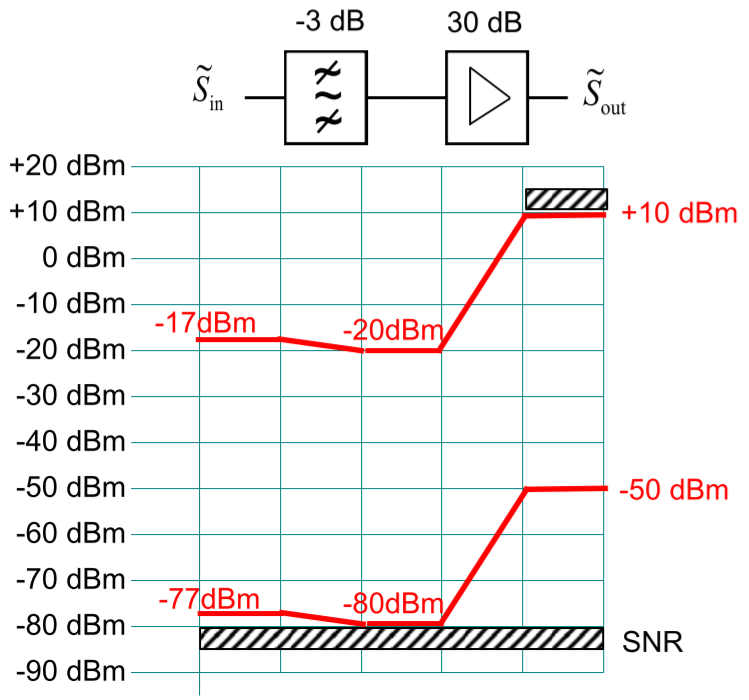
\includegraphics[width=.6\linewidth]{./11-pegelplan/hs2017}
    \vspace{-8pt}
\end{center}

\textbf{Wie gross werden gemäss des obenstehenden Pegelplans der maximale und minimale Pegel [in dBm] am Eingang des Empfängers und welche Signaldynamik [in dB] resultiert?}\\
$S_{max}=-17dBm$\\
$S_{min}=-77dBm$\\

$Signaldynamik = S_{max}-S_{min}=-17dBm+77dBm=60dB$
